\documentclass[10pt]{article}
%\documentclass[useAMS,usenatbib]{mn2e}
\usepackage{amsmath,amssymb}
\usepackage{graphicx}
\usepackage{color}
\linespread{1.05} % Line spacing
\usepackage{booktabs} % Horizontal rules in table
\usepackage{titlesec} % Allows customization of titles
\usepackage[hmarginratio=1:1,top=32mm,columnsep=20pt]{geometry} % Document margins
\usepackage[hang, small,labelfont=bf,up,textfont=it,up]{caption} % Custom captions under/above floats in tables or figures
\usepackage{float} % Required for tables and figures in the multi-column environment - they need to be placed in specific locations with the [H] (e.g. \begin{table}[H])
%\usepackage{multicol} % Used for the two-column layout of the document
\usepackage{paralist} % Used for the compactitem environment which makes bullet points with less space between them

\usepackage{hyperref} % For hyperlinks in the PDF


\renewcommand{\baselinestretch}{1}
\renewcommand{\arraystretch}{1.3}
\setlength{\topmargin}{-0.1in}
\setlength{\textheight}{8.3in}
\setlength{\oddsidemargin}{0.1 in}
\setlength{\textwidth}{6.2 in}
\usepackage{fancyhdr} % Headers and footers
\usepackage{breqn}
%\pagestyle{fancy} % All pages have headers and footers
%\fancyhead{} % Blank out the default header
%\fancyfoot{} % Blank out the default footer
%\titleformat{\section}[block]{\large\scshape\centering}{\thesection.}{1em}{} % Change the look of the section titles
%\titleformat{\subsection}[block]{\large}{\thesubsection.}{1em}{} % Change the look of the section titles
\newcommand{\done}{\hfill $\Box$ }
\newcommand{\rmap}{\stackrel{\rho}{\leftrightarrow}}
\newcommand{\mys}{\vspace{0.15in}}




\begin{document}
\bibliographystyle{abbrv}


\title{\vspace{-30mm}\fontsize{18pt}{10pt}\selectfont\textbf{Six Monthly Progress Report\\ For the period from April 2017 to November 2018  }}
\author{Gajanan D. Harale\\ Department of Physics \\ SP Pune University, Pune}

%\date{Sep 21, 2015}

 \maketitle

%\thispagestyle{plain}
%\setcounter{page}{1}
%\begin{multicols}{2} % Two-column layout throughout the main article text

\fontsize{18pt}{12pt}\selectfont\textbf{Details of Work}


%----------------------------------------------------------------------------------------


\section[]{Introduction}
\begin{itemize}
\item Two types of radio emission observed in galaxy clusters one is Relic(Peripheral Structure) other one is radio halo (central emission)
\item No proper explaination for there origin yet
\item So motivation is to find out the mechanism that can explain this two kinds of radio emission.
\item In the structure formation shocks during formation of galaxy clusters as the mechanism like Fermi one i.e. diffusive shock acceleration and second order mechanism play most vital role.
\end{itemize}
  
\section[]{Calculation of spectral index in First Order Fermi mechanism}
In fermi-1 the charged cosmic ray particles, due to the nonhomogeneous magnetic field undergo multiple encounter and each encounter it gains momentum which is equal to 
$\varepsilon P_{0}$ . So its total momentum after n encounter will be
\begin{equation}
 P_{n}= P_{0}\left( 1 + \varepsilon\right)^{n}
 \label{eq:Pn}
 \end{equation}
 
% From \ref{eq:Pn}\\ 
  $\\ln{P_{n}}=\ln{P_{0}} +n\ln{\left(1+\varepsilon\right)}$\
 
 \begin{equation}
 \therefore 
  n=\dfrac{\ln{\left(\dfrac{P_{n}}{P_{0}}\right)}}{\ln{\left(1+\varepsilon\right)}}
 \label{eq:n}
 \end{equation}
 
The probability of the cosmic ray particles to leave the magnetized plasma is $\left(p_{esc}\right)$. So the probability of cosmic ray particles in magnetized region after n-cycle is $\left( 1-p_{esc}\right)^{n}$ . 
so
\begin{equation}
 p\cong\sum_{m=n}^{+\infty}\left( 1-p_{esc}\right)^{n}
 \label{eq:sump}
\end{equation} 

%\end{table}
%\begin{table}[H]
\begin{equation}
p\cong\dfrac{\left( 1-p_{esc}\right)^{n}}{p_{esc}}
\label{eq:p}
\end{equation}


From \ref{eq:n} and \ref{eq:p}
\begin{equation}
 p\cong\dfrac{\left( 1-p_{esc}\right)^{\dfrac{\ln{\left(\dfrac{P_{n}}{P_{0}}\right)}}{\ln{\left(1+\varepsilon\right)}}}}{p_{esc}}
\label{eq:alpha}
\end{equation}
Let define
$\alpha=\dfrac{\ln{\left(\dfrac{P_{n}}{P_{0}}\right)}}{\ln{\left(1+\varepsilon\right)}}$\ \\
 %The momentum of the CR particle after n cycle is given as
 %\begin{equation}
 %P_{n}\cong\prod_{i=1}^{n}\left[1+\dfrac{4}{3}\dfrac{\left(u_{1}-u_{2}\right)}{v_{i}}\right]P_{0}
 %\label{eq:Pn1}
 %\end{equation}
% where $u_{1}$ and $u_{2}$  upstream speed and downstream speed respectively. $v$ is speed of CR particle.\\
 
 \label{eq:lnpn}
% \end{equation}
%\subsection{•}
We can write an equation 
 \begin{equation}
 f\left(P\right)=f_{0}{\left(\dfrac{P_{n}}{P_{0}}\right)}^{-\alpha}
 \label{eq:fp}
\end{equation}  
Where $ \alpha $ is the spectral index.
\section[]{Calculation of spectral index in Second Order Fermi mechanism}


Due to inhomogeneous magnetic field the energetic cosmic ray particles are scattered, which is stochastic process. Assuming the momentum distribution function $F\left(P\right)$ for energetic CR particles. Here we are considering only parallel plane shock wave case. Due to the plane parallel shock wave the CR particles undergoes $1^{st}$ order Fermi acceleration since these particles scatter back and forth across the shock. Also they undergoes $2^{nd}$ order  acceleration by turbulence. Whole process we can able to write in terms of Fokker-Planck equation.
\begin{dmath}
\frac{\partial F\left(P\right)}{\partial t}-\frac{1}{P^{2}}\frac{\partial}{\partial P}\left[P^{2}\left(\langle D\left(P\right)\rangle\frac{\partial F\left(P\right)}{\partial P}-\langle\frac{\triangle P}{\triangle T}\rangle F\left(P\right)\right)\right]+
\frac{F\left(P\right)}{\tau\left(P\right)}=Q\left(P\right)
\label{eq:fokker-planck}
\end{dmath} 
\newline And after solving it we will get the following\\
   \begin{math}
 %\begin{equation}
-\dfrac{\sigma^{2}R}{9u_{1}^{2}}\left({V_{A,1}^2}+R{V_{A,2}^2}\right)+\dfrac{\sigma R}{9u_{1}^{2}}\left[{-V_{A,1}^2}\left(3+\beta\right)-R{V_{A,1}^2}\left(3-\beta\right)\right]+\dfrac{\left(R-1\right)}{3}\sigma-\beta\dfrac{V_{A,1}^{2}R}{3u_{1}^{2}}+R=0
\label{eq:sta12}
\end{math}\\
%\end{equation}
\\Let define\\\\
$A=-\dfrac{R}{9u_{1}^{2}}\left({V_{A,1}^2}+R{V_{A,2}^2}\right)$\\
$B=\dfrac{R}{9u_{1}^{2}}\left[{-V_{A,1}^2}\left(3+\beta\right)-R{V_{A,1}^2}\left(3-\beta\right)\right]+\dfrac{\left(R-1\right)}{3}$\\
$C=-\beta\dfrac{V_{A,1}^{2}R}{3u_{1}^{2}}+R$\\ \\
 We can write
 \begin{equation}
 A\sigma^{2}+B\sigma+C=0
 \label{eq:sig}
 \end{equation}\\
 Above eq.\ref{eq:sig} has two roots which are as follows\\
 \begin{equation}
 \sigma_{1,2}=\dfrac{-B\pm \sqrt{ \left(B^{2}-4AC\right)}}{2A}
 \label{roots}
 \end{equation}
\section{Result: Simulation For Spectral index in 1st and 2nd Order Fermi mechanism}
\begin{figure}[H] \label{fig} 
  \begin{minipage}[b]{0.5\linewidth}
    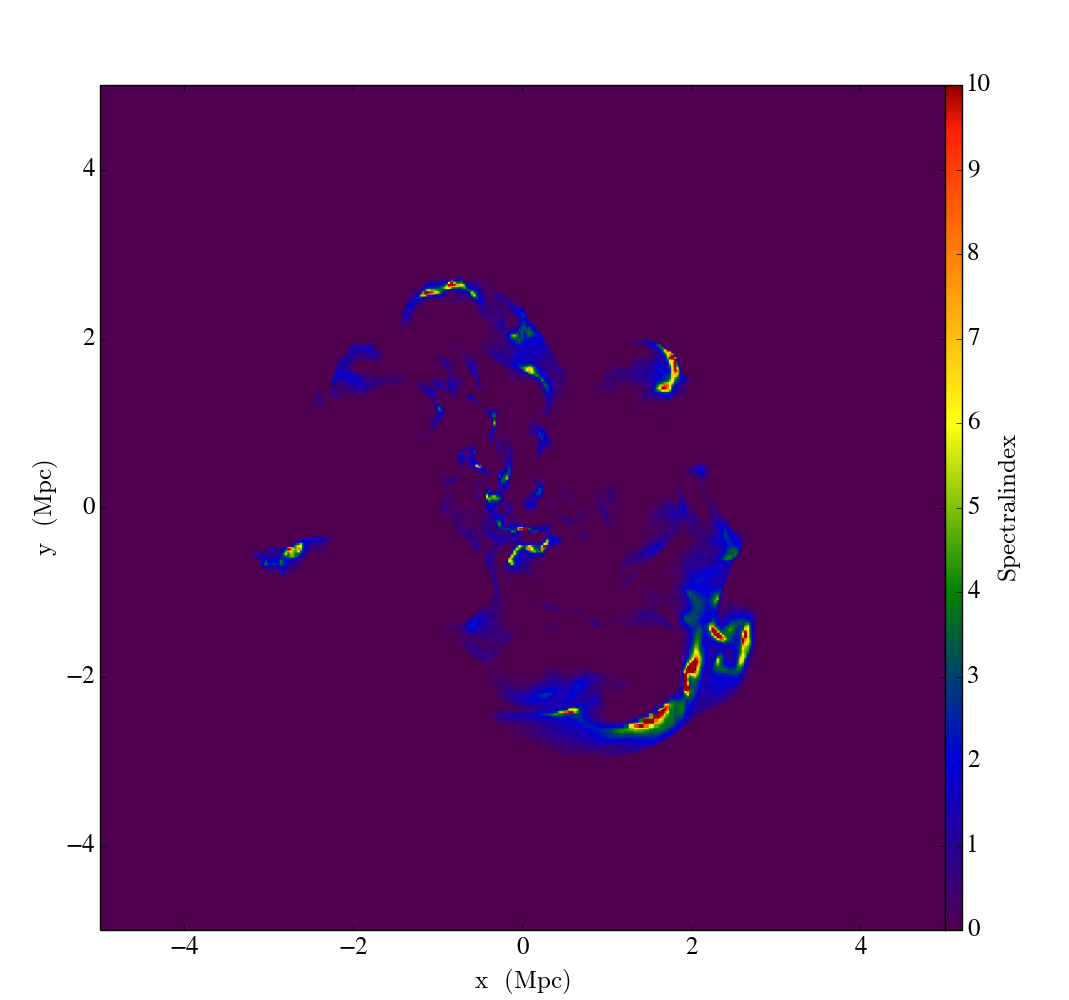
\includegraphics[width=.9\linewidth]{RedshiftOutput0033_Slice_z_SpectralIndex.png}
  \caption{Spectral Index in 1st order Fermi Mechanism} 
  \end{minipage} 
  \begin{minipage}[b]{0.5\linewidth}
    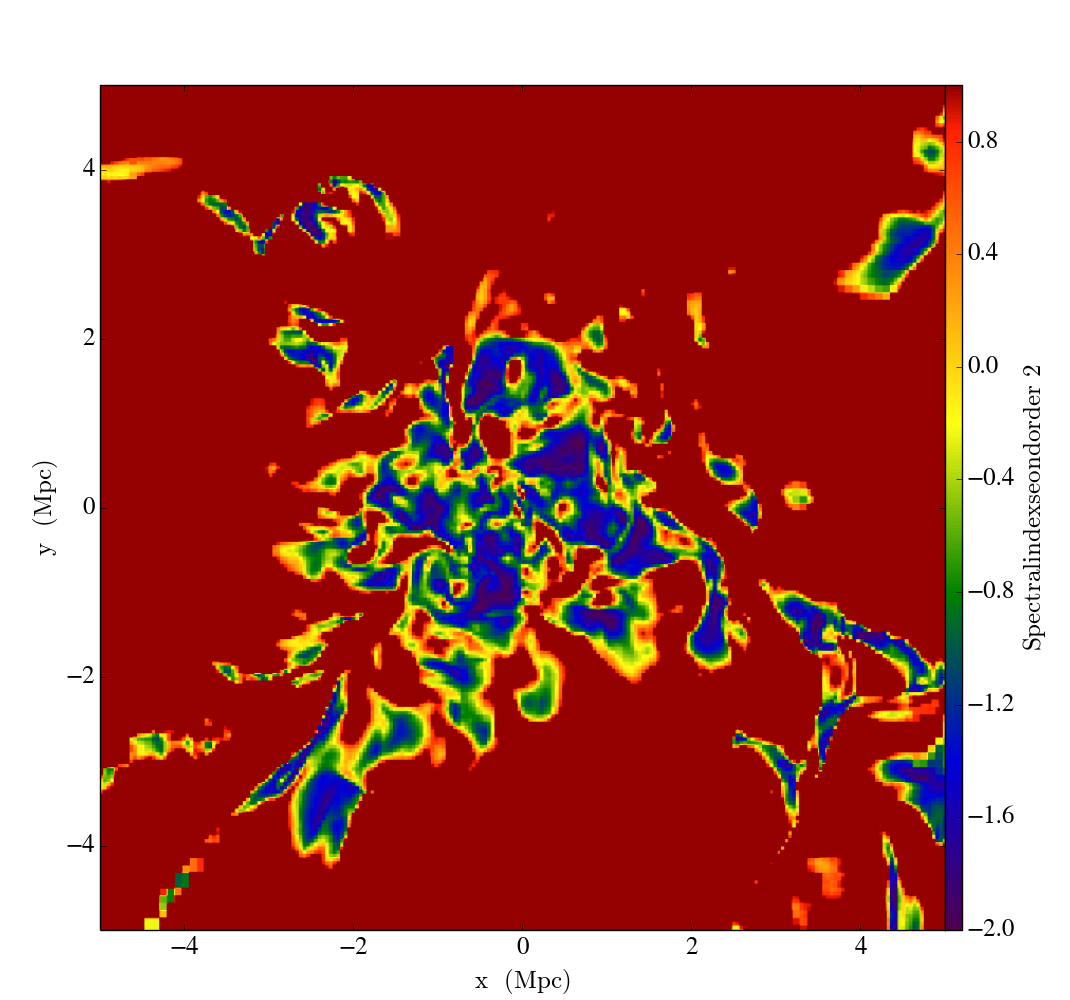
\includegraphics[width=.9\linewidth]{SpectralIndexSeondOrder_eta_2.png}
  \caption{Spectral Index in 2nd order Fermi Mechanism} 
  \end{minipage} 
  
\end{figure}

%\section*{Result}
\begin{itemize}
\item Semianalytic analysis can explain both origin of relic and halo emission.
%\item For the 1st time we computed the relative contribution from Fermi one and Fermi two mechanism to explain radio emission from galaxy clusters.
\item Fermi one or Diffusive Shock Acceleration being a strong function of mach number,significantly contributes in generating radio emission where shocks are strong and it explain the origin of radio relic.
\item Turbulence reacceleration strong function of turbulence in the medium, it is more effective central part of the cluster merger insides strong turbulence. Thus explaining the origin of radio halo.
\end{itemize}
\section{Research Publication details}[(Journal/Conferences/seminar/workshops)]
\subsection{For Conference/ seminar/ workshop : Title of the paper/abstract, authors name,
conference title, name of the organizer, duration, place.}
Title    :Forming Galaxy Clusters Are The Major Source Of Cosmic Neutrinos And Ultra
High Energy Particles\\
Author Name      : Gajanan D Harale, Dr. Surajit Paul, Reju Sam John\\
Conference Title : Young Astronomer Meet(YAM)\\
Name Of Organizer: IUCAA, Pune\\
Duration         : 11th Sept 2017 to 15th Sept 2017
\\ \\ \\ \\ \\ \\ \\ \\
\\ \\
\\ \\
\\ \\ 
\\ \\ 
\noindent\begin{tabular}{@{}p{3.5in}p{3.5in}@{}}
\dotfill                       & \dotfill\\
Signature of Student           & Signature of Guide\\
Gajanan D Harale               &  Dr. Surajit Paul
                                                           
\end{tabular} 



\end{document}
